



<!DOCTYPE html PUBLIC "-//W3C//DTD XHTML 1.0 Transitional//EN"
  "http://www.w3.org/TR/xhtml1/DTD/xhtml1-transitional.dtd">

<html xmlns="http://www.w3.org/1999/xhtml" xml:lang="en" lang="en">
  <head>
    <meta http-equiv="content-type" content="text/html;charset=UTF-8" />
        <title>ois_prj/assign2/Assignment2.tex at e060c9e7583cdee46c0e2661f08c5d0df13c6f73 from enry86's ois_prj - GitHub</title>
    <link rel="search" type="application/opensearchdescription+xml" href="/opensearch.xml" title="GitHub" />
    <link rel="fluid-icon" href="http://github.com/fluidicon.png" title="GitHub" />

    
      <link href="http://assets0.github.com/stylesheets/bundle.css?add25bbfa82f0b09a209206d69a2366544a9699b" media="screen" rel="stylesheet" type="text/css" />
    

    
      
        <script type="text/javascript" src="http://ajax.googleapis.com/ajax/libs/jquery/1.3.2/jquery.min.js"></script>
        <script src="http://assets3.github.com/javascripts/bundle.js?add25bbfa82f0b09a209206d69a2366544a9699b" type="text/javascript"></script>
      
    
    
  
    
  

  <link href="http://github.com/feeds/enry86/commits/ois_prj/e060c9e7583cdee46c0e2661f08c5d0df13c6f73" rel="alternate" title="Recent Commits to ois_prj:e060c9e7583cdee46c0e2661f08c5d0df13c6f73" type="application/atom+xml" />

  <meta name="description" content="Organizational Information Systems Project" />


    

    <script type="text/javascript">
      github_user = 'Aldebaran85'
    </script>
  </head>

  

  <body>
    

    <div id="main">
      <div id="header" class="">
        <div class="site">
          <div class="logo">
            <a href="http://github.com"><img src="/images/modules/header/logov3.png" alt="github" /></a>
          </div>
          
            <div class="topsearch">
  <form action="/search" id="top_search_form" method="get">
    <input type="search" class="search" name="q" /> <input type="submit" value="Search" />
    <input type="hidden" name="type" value="Everything" />
    <input type="hidden" name="repo" value="" />
    <input type="hidden" name="langOverride" value="" />
    <input type="hidden" name="start_value" value="1" />
  </form>
  <div class="links">
    <a href="/repositories">Browse</a> | <a href="/guides">Guides</a> | <a href="/search">Advanced</a>
  </div>
</div>
          
          
            
  <div class="corner userbox">
    <div class="box">
      <div class="gravatar">
        <a href="/"><img alt="" height="40" src="https://secure.gravatar.com/avatar/cbd1479ceb95f4b45ee33cdbb9a2a109?s=40&amp;d=http%3A%2F%2Fgithub.com%2Fimages%2Fgravatars%2Fgravatar-40.png" width="40" /></a>
      </div>

      <div class="top">
        <div class="name">
          <a href="/">Aldebaran85</a>
        </div>
        <div class="links">
          <a href="/account">account</a> |
          <a href="/Aldebaran85">profile</a> |
          <a href="/logout">log out</a>
        </div>
      </div>

      <div class="bottom">
        <div class="select">
          <div class="site_links">
                        <a href="/">dashboard</a> | <a href="http://gist.github.com/mine">gists</a>
          </div>

          <form action="/search" class="search_repos" method="get" style="display:none;">
          <input id="q" name="q" size="18" type="search" /> 
          <input type="submit" value="Search" />
          <a href="#" class="cancel_search_link">x</a>
          </form>
        </div>
        
        <div class="inbox"> <span><a href="/inbox">0</a></span> </div>
      </div>
    </div>
  </div>

          
        </div>
      </div>
      
      
        
    <div id="repo_menu">
      <div class="site">
        <ul>
          
            <li class="active"><a href="http://github.com/enry86/ois_prj/tree/">Source</a></li>

            <li class=""><a href="http://github.com/enry86/ois_prj/commits/">Commits</a></li>

            
            <li class=""><a href="/enry86/ois_prj/network">Network (0)</a></li>

            
              <li class=""><a href="/enry86/ois_prj/forkqueue">Fork Queue</a></li>
            

            
            
              
              <li class=""><a href="/enry86/ois_prj/issues">Issues (0)</a></li>
            
            

            
              
              <li class=""><a href="/enry86/ois_prj/downloads">Downloads (0)</a></li>
            

            
              
              <li class=""><a href="http://wiki.github.com/enry86/ois_prj">Wiki (1)</a></li>
            

            <li class=""><a href="/enry86/ois_prj/graphs">Graphs</a></li>

            

          
        </ul>
      </div>
    </div>

  <div id="repo_sub_menu">
    <div class="site">
      <div class="joiner"></div>
      

      

      

      
    </div>
  </div>

  <div class="site">
    





<div id="repos">
  


<script type="text/javascript">
  GitHub.currentCommitRef = "e060c9e7583cdee46c0e2661f08c5d0df13c6f73"
  GitHub.currentRepoOwner = "enry86"
  GitHub.currentRepo = "ois_prj"
</script>



  <div class="repo public">
    <div class="title">
      <div class="path">
        <a href="/enry86">enry86</a> / <b><a href="http://github.com/enry86/ois_prj/tree">ois_prj</a></b>

        

          

          
            
              
                <a href="/enry86/ois_prj/pull_request/" class="pull_request_button"><img alt="pull request" class="button" src="http://assets3.github.com/images/modules/repos/pull_request_button.png?add25bbfa82f0b09a209206d69a2366544a9699b" /></a>
              
            

            
              
                
                <a href="/enry86/ois_prj/fork"><img alt="fork" class="button" src="http://assets3.github.com/images/modules/repos/fork_button.png?add25bbfa82f0b09a209206d69a2366544a9699b" /></a>
              
            
          

          <a href="/enry86/ois_prj/toggle_watch" class="toggle_watch" style="display:none;"><img alt="watch" class="button" src="http://assets3.github.com/images/modules/repos/watch_button.png?add25bbfa82f0b09a209206d69a2366544a9699b" /></a><a href="/enry86/ois_prj/toggle_watch" class="toggle_watch"><img alt="watch" class="button" src="http://assets2.github.com/images/modules/repos/unwatch_button.png?add25bbfa82f0b09a209206d69a2366544a9699b" /></a>

          
            <a href="#" id="download_button" rel="enry86/ois_prj"><img alt="download tarball" class="button" src="http://assets2.github.com/images/modules/repos/download_button.png?add25bbfa82f0b09a209206d69a2366544a9699b" /></a>
          
        
      </div>

      <div class="security private_security" style="display:none">
        <a href="#private_repo" rel="facebox"><img src="/images/icons/private.png" alt="private" /></a>
      </div>

      <div id="private_repo" class="hidden">
        This repository is private.
        All pages are served over SSL and all pushing and pulling is done over SSH.
        No one may fork, clone, or view it unless they are added as a <a href="/enry86/ois_prj/edit">member</a>.

        <br/>
        <br/>
        Every repository with this icon (<img src="/images/icons/private.png" alt="private" />) is private.
      </div>

      <div class="security public_security" style="">
        <a href="#public_repo" rel="facebox"><img src="/images/icons/public.png" alt="public" /></a>
      </div>

      <div id="public_repo" class="hidden">
        This repository is public.
        Anyone may fork, clone, or view it.

        <br/>
        <br/>
        Every repository with this icon (<img src="/images/icons/public.png" alt="public" />) is public.
      </div>

      

        <div class="flexipill">
          <a href="/enry86/ois_prj/network">
          <table cellpadding="0" cellspacing="0">
            <tr><td><img alt="Forks" src="http://assets0.github.com/images/modules/repos/pills/forks.png?add25bbfa82f0b09a209206d69a2366544a9699b" /></td><td class="middle"><span>0</span></td><td><img alt="Right" src="http://assets1.github.com/images/modules/repos/pills/right.png?add25bbfa82f0b09a209206d69a2366544a9699b" /></td></tr>
          </table>
          </a>
        </div>

        <div class="flexipill">
          <a href="/enry86/ois_prj/watchers">
          <table cellpadding="0" cellspacing="0">
            <tr><td><img alt="Watchers" src="http://assets0.github.com/images/modules/repos/pills/watchers.png?add25bbfa82f0b09a209206d69a2366544a9699b" /></td><td class="middle"><span>2</span></td><td><img alt="Right" src="http://assets1.github.com/images/modules/repos/pills/right.png?add25bbfa82f0b09a209206d69a2366544a9699b" /></td></tr>
          </table>
          </a>
        </div>
      </div>
    
    <div class="meta">
      <table>
        
        
          <tr>
            <td class="label">Description:</td>
            <td>
              <span id="repository_description" rel="/enry86/ois_prj/edit/update" class="">Organizational Information Systems Project</span>
              
            </td>
          </tr>
        

        
          

          
            <tr>
              <td class="label">Public&nbsp;Clone&nbsp;URL:</td>
              
              <td>
                <a href="git://github.com/enry86/ois_prj.git" class="git_url_facebox" rel="#git-clone">git://github.com/enry86/ois_prj.git</a>
                      <object classid="clsid:d27cdb6e-ae6d-11cf-96b8-444553540000"
              width="110"
              height="14"
              class="clippy"
              id="clippy" >
      <param name="movie" value="/flash/clippy.swf"/>
      <param name="allowScriptAccess" value="always" />
      <param name="quality" value="high" />
      <param name="scale" value="noscale" />
      <param NAME="FlashVars" value="text=git://github.com/enry86/ois_prj.git">
      <param name="bgcolor" value="#F0F0F0">
      <param name="wmode" value="opaque">
      <embed src="/flash/clippy.swf"
             width="110"
             height="14"
             name="clippy"
             quality="high"
             allowScriptAccess="always"
             type="application/x-shockwave-flash"
             pluginspage="http://www.macromedia.com/go/getflashplayer"
             FlashVars="text=git://github.com/enry86/ois_prj.git"
             bgcolor="#F0F0F0"
             wmode="opaque"
      />
      </object>

                <div id="git-clone" style="display:none;">
                  Give this clone URL to anyone.
                  <br/>
                  <code>git clone git://github.com/enry86/ois_prj.git </code>
                </div>
              </td>
            </tr>
          
          
          <tr>
            <td class="label">Your Clone URL:</td>
            
            <td>

              <div id="private-clone-url">
                <a href="git@github.com:enry86/ois_prj.git" class="git_url_facebox" rel="#your-git-clone">git@github.com:enry86/ois_prj.git</a>
                <input type="text" value="git@github.com:enry86/ois_prj.git" style="display: none;" />
                      <object classid="clsid:d27cdb6e-ae6d-11cf-96b8-444553540000"
              width="110"
              height="14"
              class="clippy"
              id="clippy" >
      <param name="movie" value="/flash/clippy.swf"/>
      <param name="allowScriptAccess" value="always" />
      <param name="quality" value="high" />
      <param name="scale" value="noscale" />
      <param NAME="FlashVars" value="text=git@github.com:enry86/ois_prj.git">
      <param name="bgcolor" value="#F0F0F0">
      <param name="wmode" value="opaque">
      <embed src="/flash/clippy.swf"
             width="110"
             height="14"
             name="clippy"
             quality="high"
             allowScriptAccess="always"
             type="application/x-shockwave-flash"
             pluginspage="http://www.macromedia.com/go/getflashplayer"
             FlashVars="text=git@github.com:enry86/ois_prj.git"
             bgcolor="#F0F0F0"
             wmode="opaque"
      />
      </object>

              </div>

              <div id="your-git-clone" style="display:none;">
                Use this clone URL yourself.
                <br/>
                <code>git clone git@github.com:enry86/ois_prj.git </code>
              </div>
            </td>
          </tr>
          
          

          

          
      </table>

          </div>
  </div>






</div>


  <div id="commit">
    <div class="group">
        
  <div class="envelope commit">
    <div class="human">
      
        <div class="message"><pre><a href="/enry86/ois_prj/commit/e060c9e7583cdee46c0e2661f08c5d0df13c6f73">added course management</a> </pre></div>
      

      <div class="actor">
        <div class="gravatar">
          
          <img alt="" height="30" src="http://www.gravatar.com/avatar/89e94b16c91e56fc49f83f04d80919a7?s=30&amp;d=http%3A%2F%2Fgithub.com%2Fimages%2Fgravatars%2Fgravatar-30.png" width="30" />
        </div>
        <div class="name"><a href="/enry86">enry86</a> <span>(author)</span></div>
          <div class="date">
            <abbr class="relatize" title="2009-05-03 15:49:37">Sun May 03 15:49:37 -0700 2009</abbr> 
          </div>
      </div>
  
      
  
    </div>
    <div class="machine">
      <span>c</span>ommit&nbsp;&nbsp;<a href="/enry86/ois_prj/commit/e060c9e7583cdee46c0e2661f08c5d0df13c6f73" hotkey="c">e060c9e7583cdee46c0e2661f08c5d0df13c6f73</a><br />
      <span>t</span>ree&nbsp;&nbsp;&nbsp;&nbsp;<a href="/enry86/ois_prj/tree/e060c9e7583cdee46c0e2661f08c5d0df13c6f73" hotkey="t">0405e83c6304b469629128dfbbbbff238c70855b</a><br />
  
      
        <span>p</span>arent&nbsp;
        
        <a href="/enry86/ois_prj/tree/2162bead2e65a1372bc30ab7e51b8a42cba8650d" hotkey="p">2162bead2e65a1372bc30ab7e51b8a42cba8650d</a>
      
  
    </div>
  </div>

    </div>
  </div>



  
    <div id="path">
      <b><a href="/enry86/ois_prj/tree">ois_prj</a></b> / <a href="/enry86/ois_prj/tree/e060c9e7583cdee46c0e2661f08c5d0df13c6f73/ois_prj">ois_prj</a> / <a href="/enry86/ois_prj/tree/e060c9e7583cdee46c0e2661f08c5d0df13c6f73/ois_prj/assign2">assign2</a> / Assignment2.tex       <object classid="clsid:d27cdb6e-ae6d-11cf-96b8-444553540000"
              width="110"
              height="14"
              class="clippy"
              id="clippy" >
      <param name="movie" value="/flash/clippy.swf"/>
      <param name="allowScriptAccess" value="always" />
      <param name="quality" value="high" />
      <param name="scale" value="noscale" />
      <param NAME="FlashVars" value="text=ois_prj/assign2/Assignment2.tex">
      <param name="bgcolor" value="#FFFFFF">
      <param name="wmode" value="opaque">
      <embed src="/flash/clippy.swf"
             width="110"
             height="14"
             name="clippy"
             quality="high"
             allowScriptAccess="always"
             type="application/x-shockwave-flash"
             pluginspage="http://www.macromedia.com/go/getflashplayer"
             FlashVars="text=ois_prj/assign2/Assignment2.tex"
             bgcolor="#FFFFFF"
             wmode="opaque"
      />
      </object>

    </div>

    <div id="files">
      <div class="file">
        <div class="meta">
          <div class="info">
            <span>100644</span>
            <span>104 lines (89 sloc)</span>
            <span>4.982 kb</span>
          </div>
          <div class="actions">
            
              <a id="file-edit-link" href="#" rel="/enry86/ois_prj/file-edit/e060c9e7583cdee46c0e2661f08c5d0df13c6f73/ois_prj/assign2/Assignment2.tex">edit</a>
            
            <a href="/enry86/ois_prj/raw/e060c9e7583cdee46c0e2661f08c5d0df13c6f73/ois_prj/assign2/Assignment2.tex" id="raw-url">raw</a>
            
              <a href="/enry86/ois_prj/blame/e060c9e7583cdee46c0e2661f08c5d0df13c6f73/ois_prj/assign2/Assignment2.tex">blame</a>
            
            <a href="/enry86/ois_prj/commits/master/ois_prj/assign2/Assignment2.tex">history</a>
          </div>
        </div>
        
  <div class="data syntax">
    
      <table cellpadding="0" cellspacing="0">
        <tr>
          <td>
            
            <pre class="line_numbers">
<span id="LID1" rel="#L1">1</span>
<span id="LID2" rel="#L2">2</span>
<span id="LID3" rel="#L3">3</span>
<span id="LID4" rel="#L4">4</span>
<span id="LID5" rel="#L5">5</span>
<span id="LID6" rel="#L6">6</span>
<span id="LID7" rel="#L7">7</span>
<span id="LID8" rel="#L8">8</span>
<span id="LID9" rel="#L9">9</span>
<span id="LID10" rel="#L10">10</span>
<span id="LID11" rel="#L11">11</span>
<span id="LID12" rel="#L12">12</span>
<span id="LID13" rel="#L13">13</span>
<span id="LID14" rel="#L14">14</span>
<span id="LID15" rel="#L15">15</span>
<span id="LID16" rel="#L16">16</span>
<span id="LID17" rel="#L17">17</span>
<span id="LID18" rel="#L18">18</span>
<span id="LID19" rel="#L19">19</span>
<span id="LID20" rel="#L20">20</span>
<span id="LID21" rel="#L21">21</span>
<span id="LID22" rel="#L22">22</span>
<span id="LID23" rel="#L23">23</span>
<span id="LID24" rel="#L24">24</span>
<span id="LID25" rel="#L25">25</span>
<span id="LID26" rel="#L26">26</span>
<span id="LID27" rel="#L27">27</span>
<span id="LID28" rel="#L28">28</span>
<span id="LID29" rel="#L29">29</span>
<span id="LID30" rel="#L30">30</span>
<span id="LID31" rel="#L31">31</span>
<span id="LID32" rel="#L32">32</span>
<span id="LID33" rel="#L33">33</span>
<span id="LID34" rel="#L34">34</span>
<span id="LID35" rel="#L35">35</span>
<span id="LID36" rel="#L36">36</span>
<span id="LID37" rel="#L37">37</span>
<span id="LID38" rel="#L38">38</span>
<span id="LID39" rel="#L39">39</span>
<span id="LID40" rel="#L40">40</span>
<span id="LID41" rel="#L41">41</span>
<span id="LID42" rel="#L42">42</span>
<span id="LID43" rel="#L43">43</span>
<span id="LID44" rel="#L44">44</span>
<span id="LID45" rel="#L45">45</span>
<span id="LID46" rel="#L46">46</span>
<span id="LID47" rel="#L47">47</span>
<span id="LID48" rel="#L48">48</span>
<span id="LID49" rel="#L49">49</span>
<span id="LID50" rel="#L50">50</span>
<span id="LID51" rel="#L51">51</span>
<span id="LID52" rel="#L52">52</span>
<span id="LID53" rel="#L53">53</span>
<span id="LID54" rel="#L54">54</span>
<span id="LID55" rel="#L55">55</span>
<span id="LID56" rel="#L56">56</span>
<span id="LID57" rel="#L57">57</span>
<span id="LID58" rel="#L58">58</span>
<span id="LID59" rel="#L59">59</span>
<span id="LID60" rel="#L60">60</span>
<span id="LID61" rel="#L61">61</span>
<span id="LID62" rel="#L62">62</span>
<span id="LID63" rel="#L63">63</span>
<span id="LID64" rel="#L64">64</span>
<span id="LID65" rel="#L65">65</span>
<span id="LID66" rel="#L66">66</span>
<span id="LID67" rel="#L67">67</span>
<span id="LID68" rel="#L68">68</span>
<span id="LID69" rel="#L69">69</span>
<span id="LID70" rel="#L70">70</span>
<span id="LID71" rel="#L71">71</span>
<span id="LID72" rel="#L72">72</span>
<span id="LID73" rel="#L73">73</span>
<span id="LID74" rel="#L74">74</span>
<span id="LID75" rel="#L75">75</span>
<span id="LID76" rel="#L76">76</span>
<span id="LID77" rel="#L77">77</span>
<span id="LID78" rel="#L78">78</span>
<span id="LID79" rel="#L79">79</span>
<span id="LID80" rel="#L80">80</span>
<span id="LID81" rel="#L81">81</span>
<span id="LID82" rel="#L82">82</span>
<span id="LID83" rel="#L83">83</span>
<span id="LID84" rel="#L84">84</span>
<span id="LID85" rel="#L85">85</span>
<span id="LID86" rel="#L86">86</span>
<span id="LID87" rel="#L87">87</span>
<span id="LID88" rel="#L88">88</span>
<span id="LID89" rel="#L89">89</span>
<span id="LID90" rel="#L90">90</span>
<span id="LID91" rel="#L91">91</span>
<span id="LID92" rel="#L92">92</span>
<span id="LID93" rel="#L93">93</span>
<span id="LID94" rel="#L94">94</span>
<span id="LID95" rel="#L95">95</span>
<span id="LID96" rel="#L96">96</span>
<span id="LID97" rel="#L97">97</span>
<span id="LID98" rel="#L98">98</span>
<span id="LID99" rel="#L99">99</span>
<span id="LID100" rel="#L100">100</span>
<span id="LID101" rel="#L101">101</span>
<span id="LID102" rel="#L102">102</span>
<span id="LID103" rel="#L103">103</span>
<span id="LID104" rel="#L104">104</span>
</pre>
          </td>
          <td width="100%">
            
            
              <div class="highlight"><pre><div class="line" id="LC1"><span class="k">\chapter</span><span class="nb">{</span>Business Processes<span class="nb">}</span></div><div class="line" id="LC2">In this chapter we analyze a set of business processes which are</div><div class="line" id="LC3">fundamental activities inside our organization, we provide an analysis of</div><div class="line" id="LC4">these processes and the results of a simulation.</div><div class="line" id="LC5">&nbsp;</div><div class="line" id="LC6">Before going in deeper details in analyzing the processes is useful to get</div><div class="line" id="LC7">a wider view on the organization structure.</div><div class="line" id="LC8">AllSpark, is an enterprise with the aim to develop and deploy services in</div><div class="line" id="LC9">the IT area.</div><div class="line" id="LC10">&nbsp;</div><div class="line" id="LC11">Our products can vary from a common web hosting service to very complex and</div><div class="line" id="LC12">possibly innovative security systems, and therefore we need to distinguish</div><div class="line" id="LC13">the different departments in which our organization is divided.</div><div class="line" id="LC14">&nbsp;</div><div class="line" id="LC15"><span class="k">\section</span><span class="nb">{</span>Departments and structure<span class="nb">}</span></div><div class="line" id="LC16">AllSpark organization is divided in several activity areas, each one of them</div><div class="line" id="LC17">contains the processes and the people needed to operate in a specific</div><div class="line" id="LC18">field. </div><div class="line" id="LC19">&nbsp;</div><div class="line" id="LC20">For a more detailed view on the organization is useful to provide a</div><div class="line" id="LC21">formalization of these concepts, through a set of diagrams which are going</div><div class="line" id="LC22">to be described in the following sections. In particular the attention has</div><div class="line" id="LC23">been focused in representing the two sides of the organization: first it&#39;s</div><div class="line" id="LC24">possible to analyze which are the different roles inside the company and</div><div class="line" id="LC25">how they are distributed, then is presented a view on which business</div><div class="line" id="LC26">processes are involved in the different areas of the company.</div><div class="line" id="LC27">&nbsp;</div><div class="line" id="LC28"><span class="k">\subsection</span><span class="nb">{</span>Working structure<span class="nb">}</span></div><div class="line" id="LC29">The working structure represent the general structure of AllSpark internal</div><div class="line" id="LC30">organization. For simplicity the number of employees is not represented</div><div class="line" id="LC31">since there may be several entities for each &quot;Performer&quot; depending on the</div><div class="line" id="LC32">working load and on the size of the projects involved. Each performer is a</div><div class="line" id="LC33">facet entity since several people may collaborate in that position to reach</div><div class="line" id="LC34">the Roles defined, but identifying all of them with a single term and</div><div class="line" id="LC35">element in the structure, permits a simpler representation of the concept.</div><div class="line" id="LC36">&nbsp;</div><div class="line" id="LC37">The two main areas, Administrative and Research and Development, distinguish</div><div class="line" id="LC38">the scope the employee would reach. In the former the main interest is</div><div class="line" id="LC39">directly connected to the set of functions which permits the right and</div><div class="line" id="LC40">complete Company lifecycle. The latter is bind to the Company productivity,</div><div class="line" id="LC41">that are the basic elements which are involved in the growing of</div><div class="line" id="LC42">the invoice.</div><div class="line" id="LC43">&nbsp;</div><div class="line" id="LC44">The Working Team is an abstract organizational unit which represent a group</div><div class="line" id="LC45">of employee which are involved in a particular project, or in some some</div><div class="line" id="LC46">cases in different ones, that need different skills and knowledges to be</div><div class="line" id="LC47">developed. In the organization there may be several Working Team in order to</div><div class="line" id="LC48">maximize the performance in productivity and in the Project management.</div><div class="line" id="LC49">&nbsp;</div><div class="line" id="LC50">The Public Relation organizational unit aims to represent the group of</div><div class="line" id="LC51">people who are charged to represent the Company in meetings, in the</div><div class="line" id="LC52">approaching with customers and for consulting.</div><div class="line" id="LC53">&nbsp;</div><div class="line" id="LC54">Figure <span class="k">\ref</span><span class="nb">{</span>2img:working<span class="nb">}</span> can describe in details how people working for</div><div class="line" id="LC55">AllSpark is organized inside the company.</div><div class="line" id="LC56">&nbsp;</div><div class="line" id="LC57"><span class="k">\begin</span><span class="nb">{</span>figure<span class="nb">}</span></div><div class="line" id="LC58"><span class="k">\begin</span><span class="nb">{</span>centering<span class="nb">}</span></div><div class="line" id="LC59"><span class="k">\includegraphics</span><span class="na">[scale=0.45]</span><span class="nb">{</span>assign2/adonis/imgs/working<span class="nb">_</span>structure.jpg<span class="nb">}</span></div><div class="line" id="LC60"><span class="k">\caption</span><span class="nb">{</span>AllSpark working structure<span class="nb">}</span></div><div class="line" id="LC61"><span class="k">\label</span><span class="nb">{</span>2img:working<span class="nb">}</span></div><div class="line" id="LC62"><span class="k">\end</span><span class="nb">{</span>centering<span class="nb">}</span></div><div class="line" id="LC63"><span class="k">\end</span><span class="nb">{</span>figure<span class="nb">}</span></div><div class="line" id="LC64">&nbsp;</div><div class="line" id="LC65"><span class="k">\subsection</span><span class="nb">{</span>Company organization<span class="nb">}</span></div><div class="line" id="LC66">In the AllSpark organization is possible to identify the following</div><div class="line" id="LC67">different areas:</div><div class="line" id="LC68"><span class="k">\begin</span><span class="nb">{</span>description<span class="nb">}</span></div><div class="line" id="LC69"><span class="k">\item</span><span class="na">[Administration:]</span> This part of the enterprise manages the</div><div class="line" id="LC70">administrative part of the organization, takes marketing decision, follows</div><div class="line" id="LC71">the public relations with external partners, solves bureaucratic issues</div><div class="line" id="LC72">and is responsible for the financial operations.</div><div class="line" id="LC73"><span class="k">\item</span><span class="na">[Project Management:]</span> This segment of the organization is involved in</div><div class="line" id="LC74">the core processes of manage the different phases of project development.</div><div class="line" id="LC75">These activities represent a set of core functions in the organizations</div><div class="line" id="LC76">aims, is this sector, in facts, which is responsible for the actual</div><div class="line" id="LC77">implementation of our products.</div><div class="line" id="LC78"><span class="k">\item</span><span class="na">[Working resource management:]</span> The processes and resources which are</div><div class="line" id="LC79">involved in this sector provide support for the maintenance of hardware</div><div class="line" id="LC80">and software. There are processes dedicated to reparation as to the update</div><div class="line" id="LC81">of different resources.</div><div class="line" id="LC82"><span class="k">\item</span><span class="na">[Course and Certification:]</span> AllSpark, as an enterprise, organizes</div><div class="line" id="LC83">courses for developers and sysadmins. For this reason a particular division</div><div class="line" id="LC84">of the organization is dedicated to the management of courses and seminars.</div><div class="line" id="LC85"><span class="k">\item</span><span class="na">[Research and Development:]</span> The employees in this area work actively in</div><div class="line" id="LC86">the research&#39;s world, mainly in security related field. In our organization</div><div class="line" id="LC87">this section is vital for improving our products and develop new one.</div><div class="line" id="LC88"><span class="k">\end</span><span class="nb">{</span>description<span class="nb">}</span></div><div class="line" id="LC89">&nbsp;</div><div class="line" id="LC90">The company map in figure <span class="k">\ref</span><span class="nb">{</span>2img:cmap<span class="nb">}</span> depicts clearly the business processes</div><div class="line" id="LC91">performed in each section and how them are related to each other.</div><div class="line" id="LC92">&nbsp;</div><div class="line" id="LC93"><span class="k">\begin</span><span class="nb">{</span>figure<span class="nb">}</span></div><div class="line" id="LC94"><span class="k">\begin</span><span class="nb">{</span>centering<span class="nb">}</span></div><div class="line" id="LC95"><span class="k">\includegraphics</span><span class="na">[scale=0.43]</span><span class="nb">{</span>assign2/adonis/imgs/companymap.jpg<span class="nb">}</span></div><div class="line" id="LC96"><span class="k">\caption</span><span class="nb">{</span>AllSpark company map<span class="nb">}</span></div><div class="line" id="LC97"><span class="k">\label</span><span class="nb">{</span>2img:cmap<span class="nb">}</span></div><div class="line" id="LC98"><span class="k">\end</span><span class="nb">{</span>centering<span class="nb">}</span></div><div class="line" id="LC99"><span class="k">\end</span><span class="nb">{</span>figure<span class="nb">}</span></div><div class="line" id="LC100">&nbsp;</div><div class="line" id="LC101"><span class="c">%\subsection{Login}

\begin{figure}
\begin{centering}
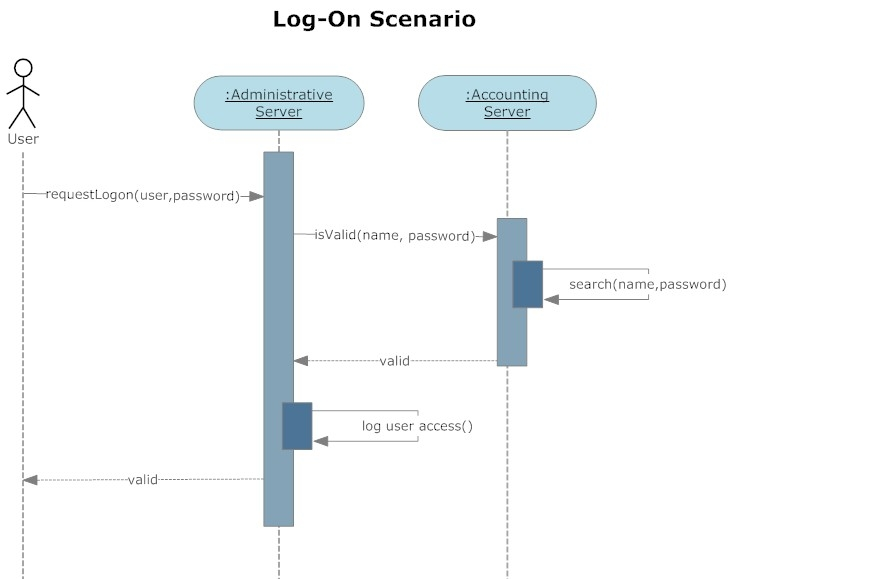
\includegraphics[scale=0.45]{assign3/sdraw/imgs/login.jpg}
\caption{Login sequence diagram.}
\label{3img:[sequence]login}
\end{centering}
\end{figure}

\subsection{Sending order}
\begin{figure}
\begin{centering}
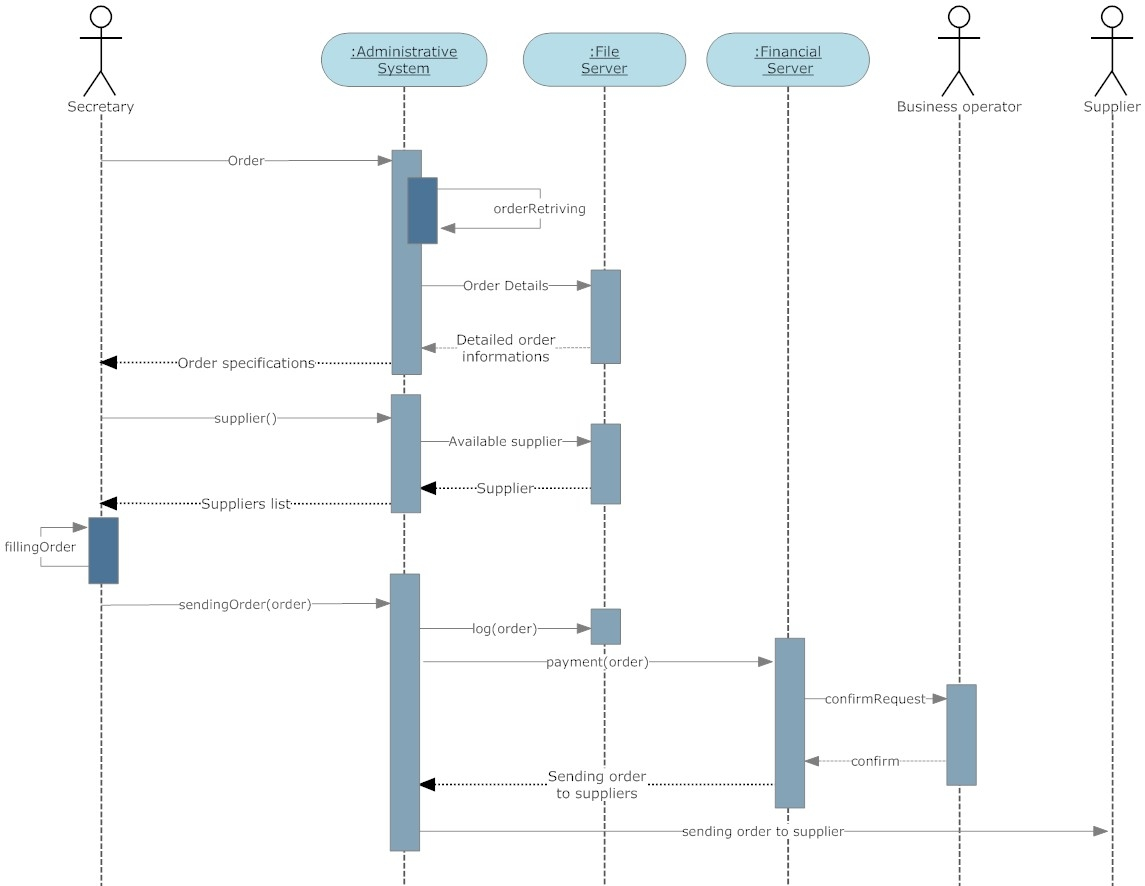
\includegraphics[scale=0.45,angle=90]{assign3/sdraw/imgs/sending_order.jpg}
\caption{Sending order sequence diagram.}
\label{3img:[sequence]sending_order}
\end{centering}
\end{figure}

\subsection{Maintenance schedule}
\begin{figure}
\begin{centering}
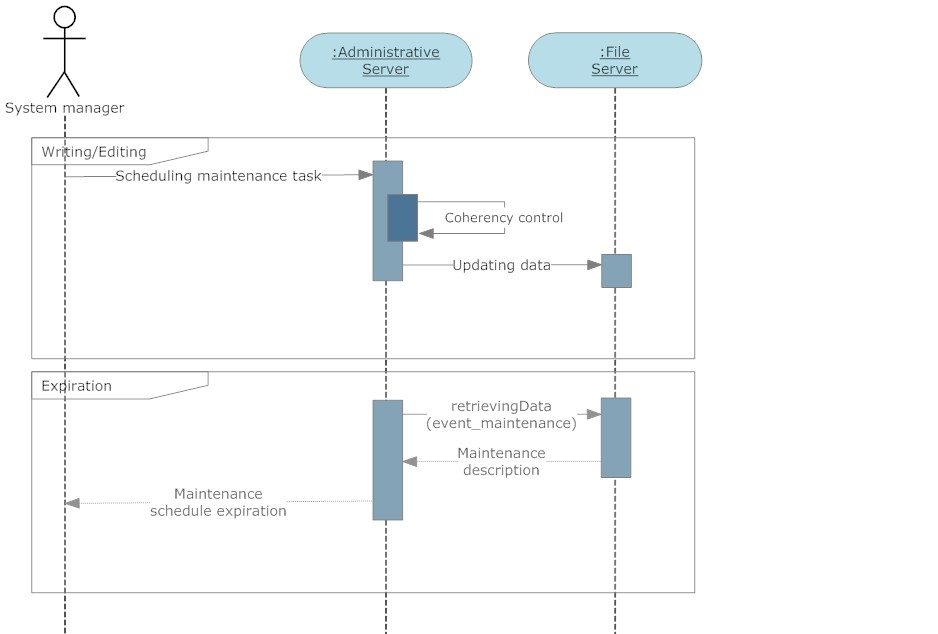
\includegraphics[scale=0.50]{assign3/sdraw/imgs/maintenance.jpg}
\caption{Maintenance schedule sequence diagram.}
\label{3img:[sequence]maintenance}
\end{centering}
\end{figure}

\subsection{Meeting management}
\begin{figure}
\begin{centering}
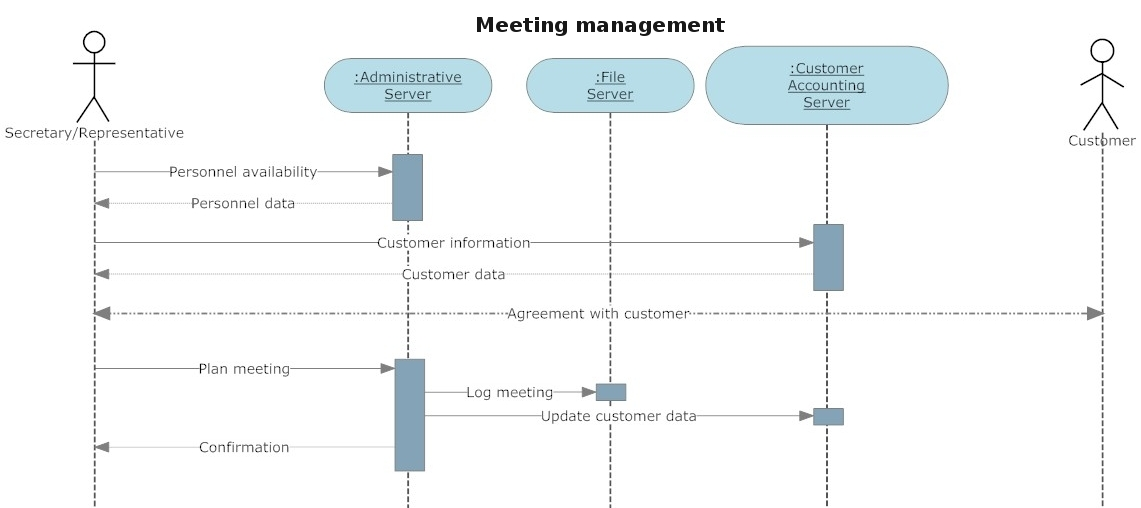
\includegraphics[scale=0.35]{assign3/sdraw/imgs/meeting.jpg}
\caption{Meeting management sequence diagram.}
\label{3img:[sequence]meeting}
\end{centering}
\end{figure}

\subsection{Project planning}
\begin{figure}
\begin{centering}
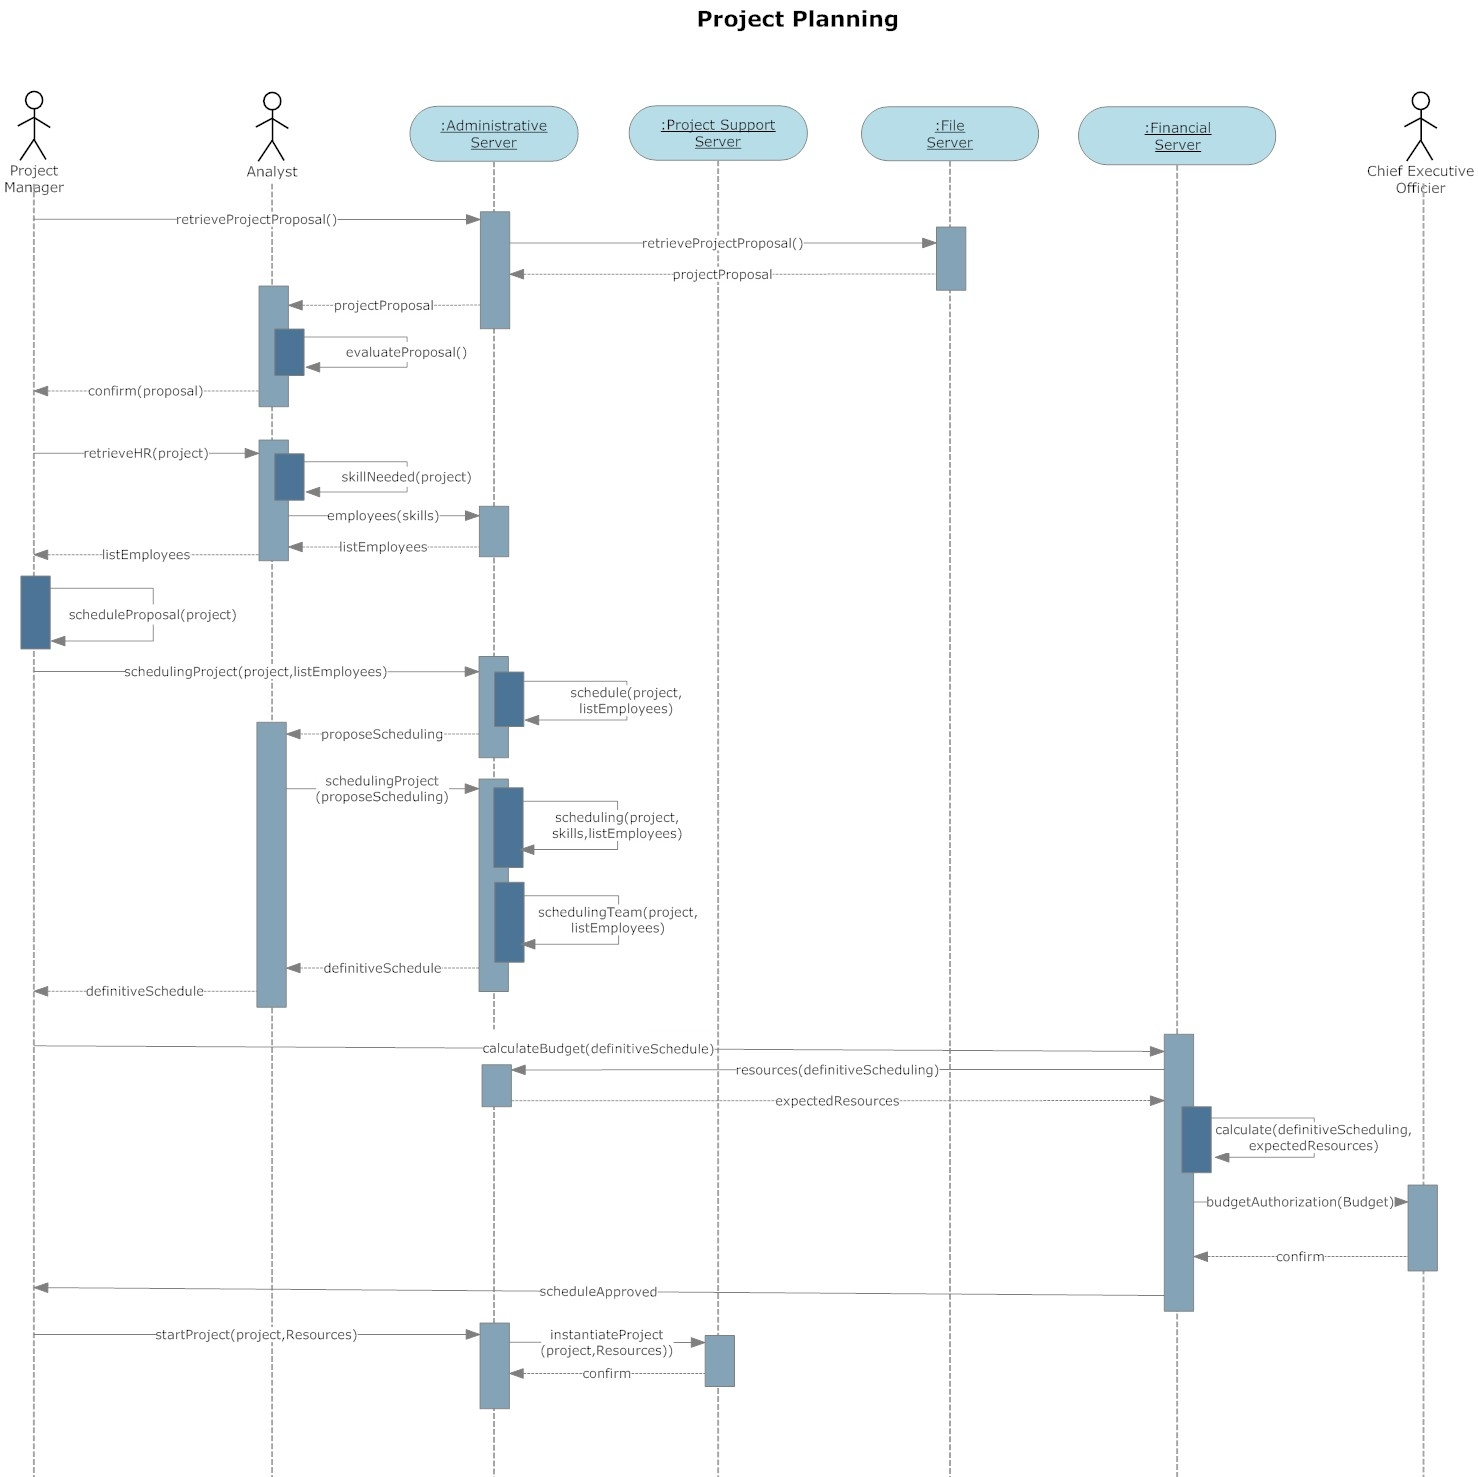
\includegraphics[scale=0.30,angle=90]{assign3/sdraw/imgs/project_planning.jpg}
\caption{Project planning sequence diagram.}
\label{3img:[sequence]project_planning}
\end{centering}
\end{figure}

\subsection{Checking work}
\begin{figure}
\begin{centering}
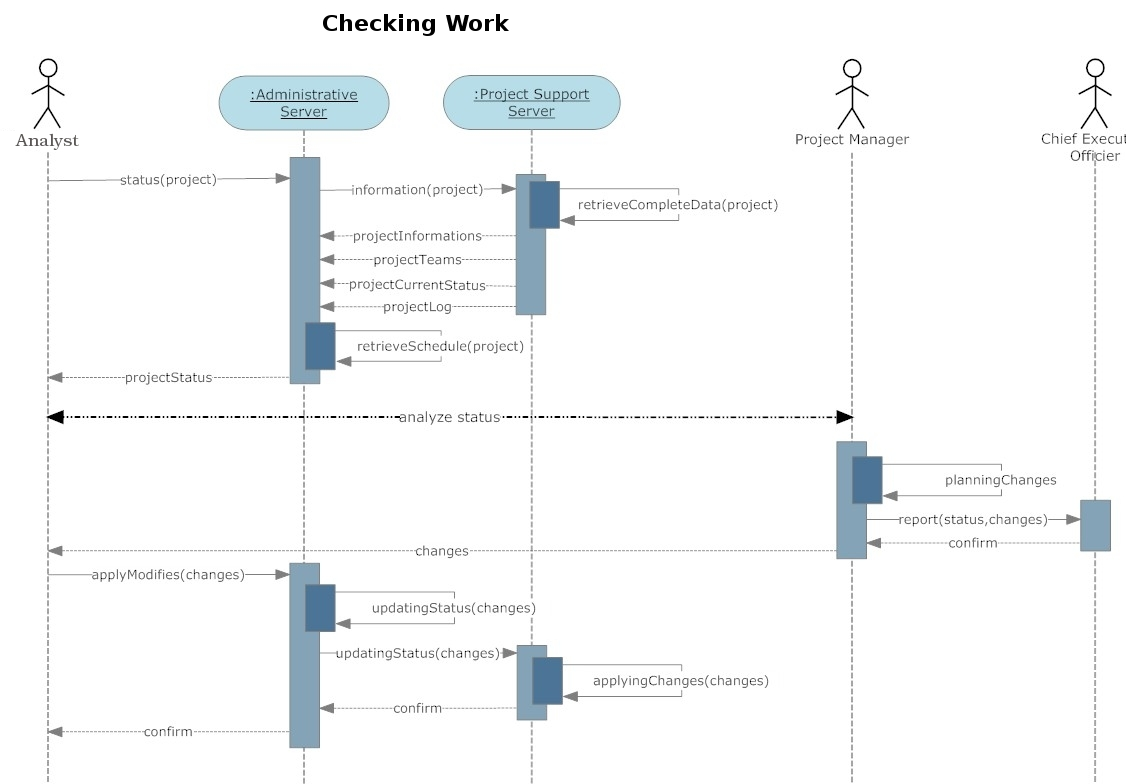
\includegraphics[scale=0.35]{assign3/sdraw/imgs/checking.jpg}
\caption{Checking work sequence diagram.}
\label{3img:[sequence]checking}
\end{centering}
\end{figure}

\subsection{Team monitoring}
\begin{figure}
\begin{centering}
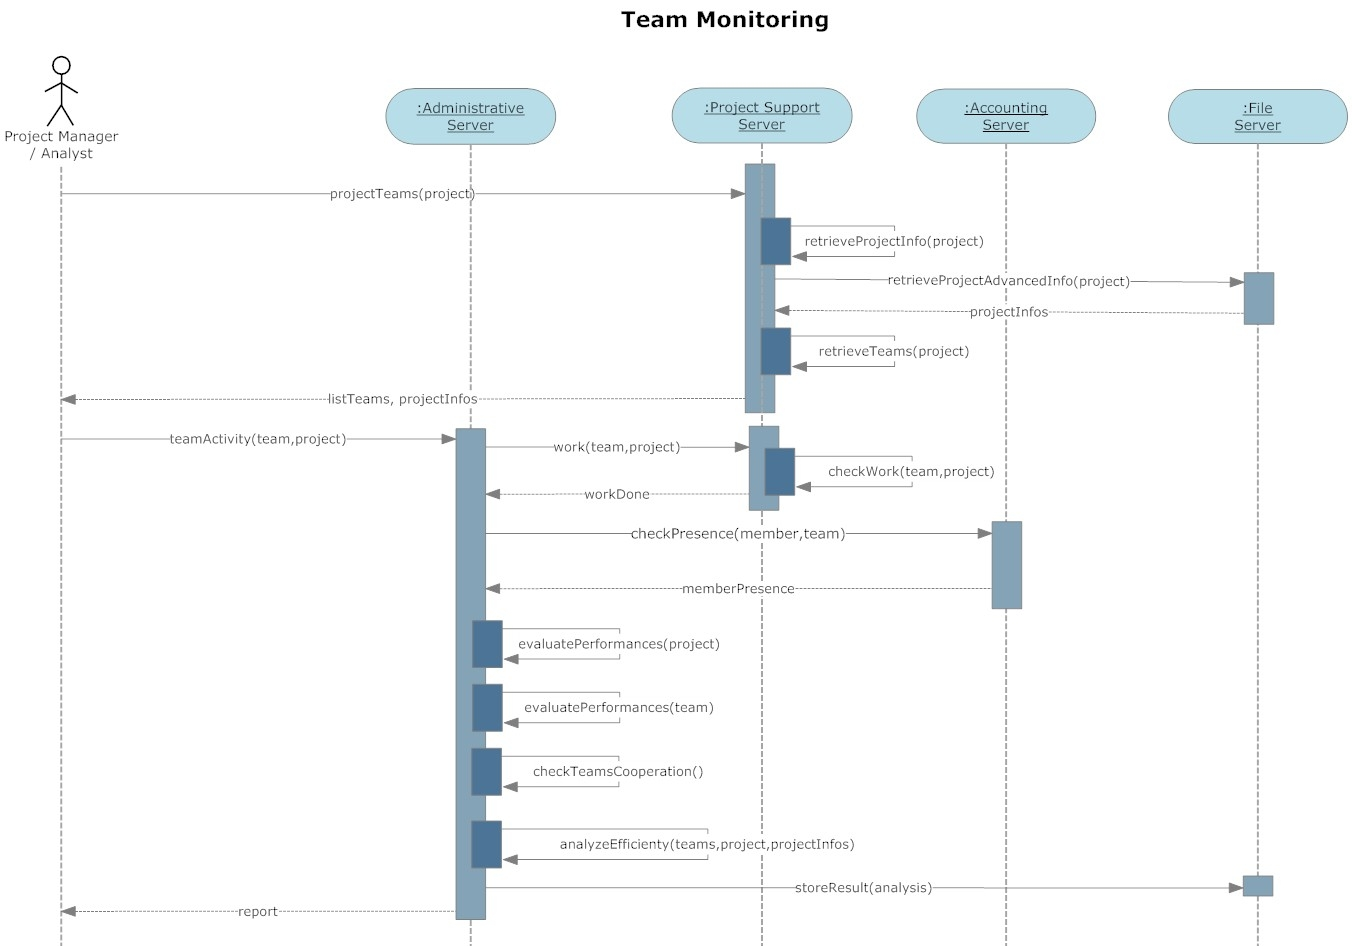
\includegraphics[scale=0.40,angle=90]{assign3/sdraw/imgs/team_monitoring.jpg}
\caption{Team monitoring sequence diagram.}
\label{3img:[sequence]team_monitoring}
\end{centering}
\end{figure}

\subsection{Course log}
\begin{figure}
\begin{centering}
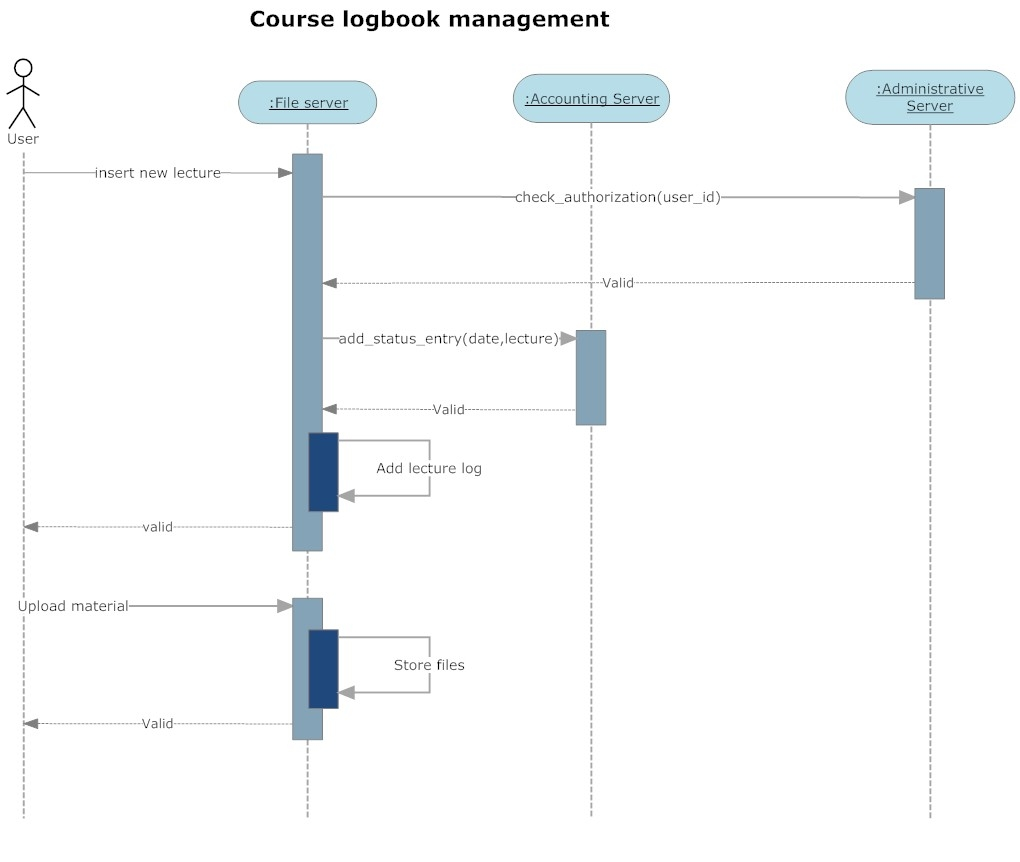
\includegraphics[scale=0.45]{assign3/sdraw/imgs/course_log.jpg}
\caption{Course log sequence diagram.}
\label{3img:[sequence]course_log}
\end{centering}
\end{figure}

\subsection{Certification}
\begin{figure}
\begin{centering}
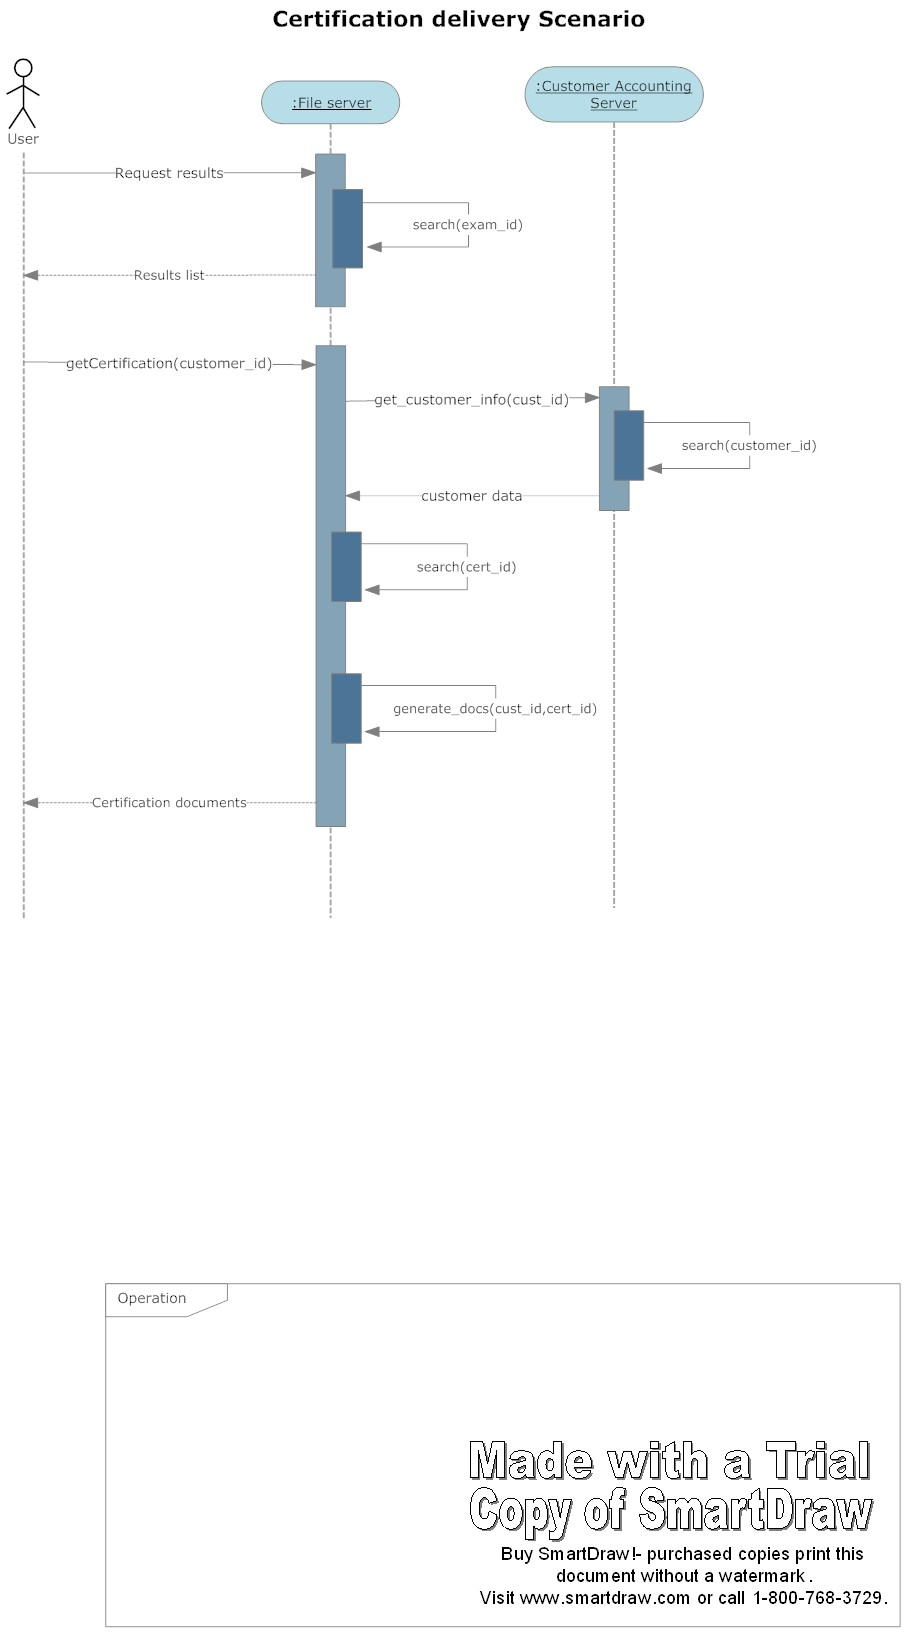
\includegraphics[scale=0.55]{assign3/sdraw/imgs/certification.jpg}
\caption{Certification sequence diagram.}
\label{3img:[sequence]certification}
\end{centering}
\end{figure}

\subsection{Campaign planning}
\begin{figure}
\begin{centering}
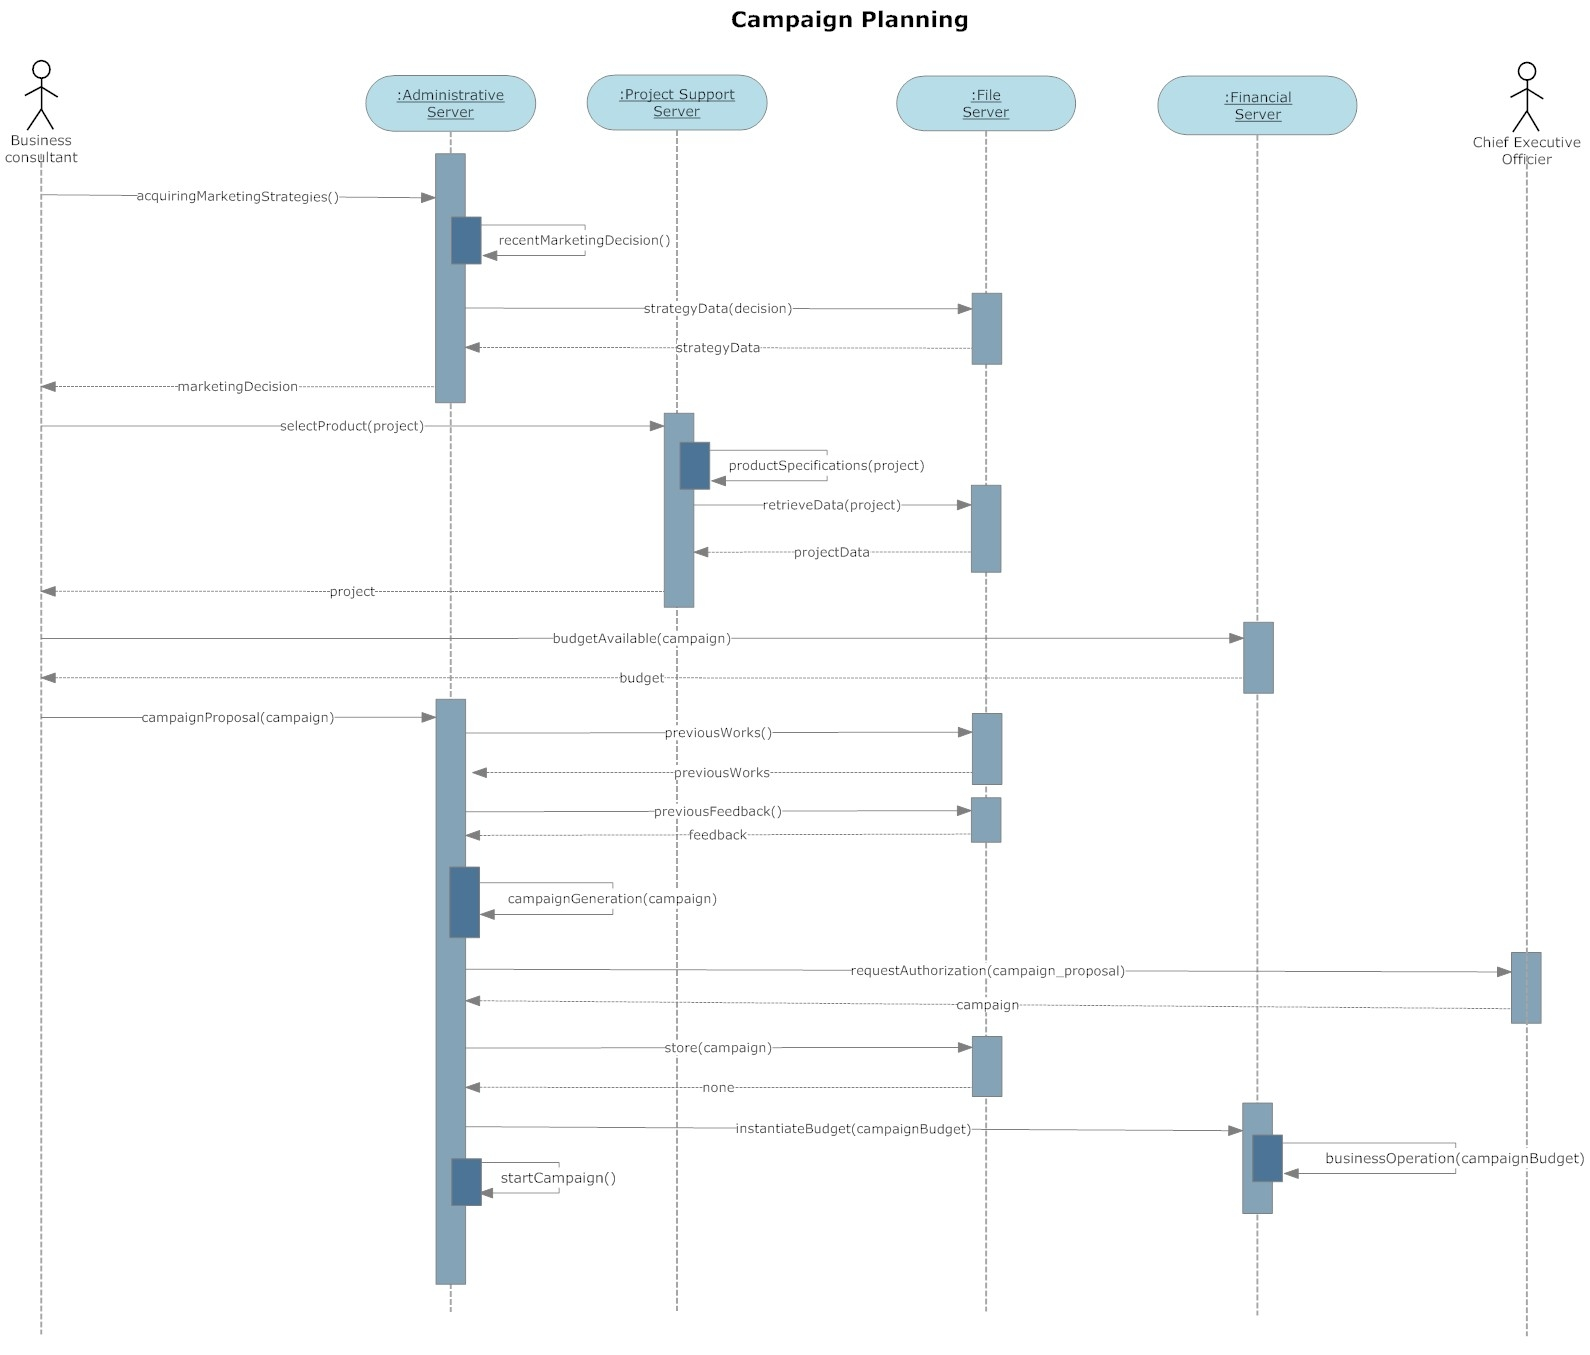
\includegraphics[scale=0.35,angle=90]{assign3/sdraw/imgs/campaign_planning.jpg}
\caption{Campaign planning sequence diagram.}
\label{3img:[sequence]campaign_planning}
\end{centering}
\end{figure}

\subsection{Inventory management}
\begin{figure}
\begin{centering}
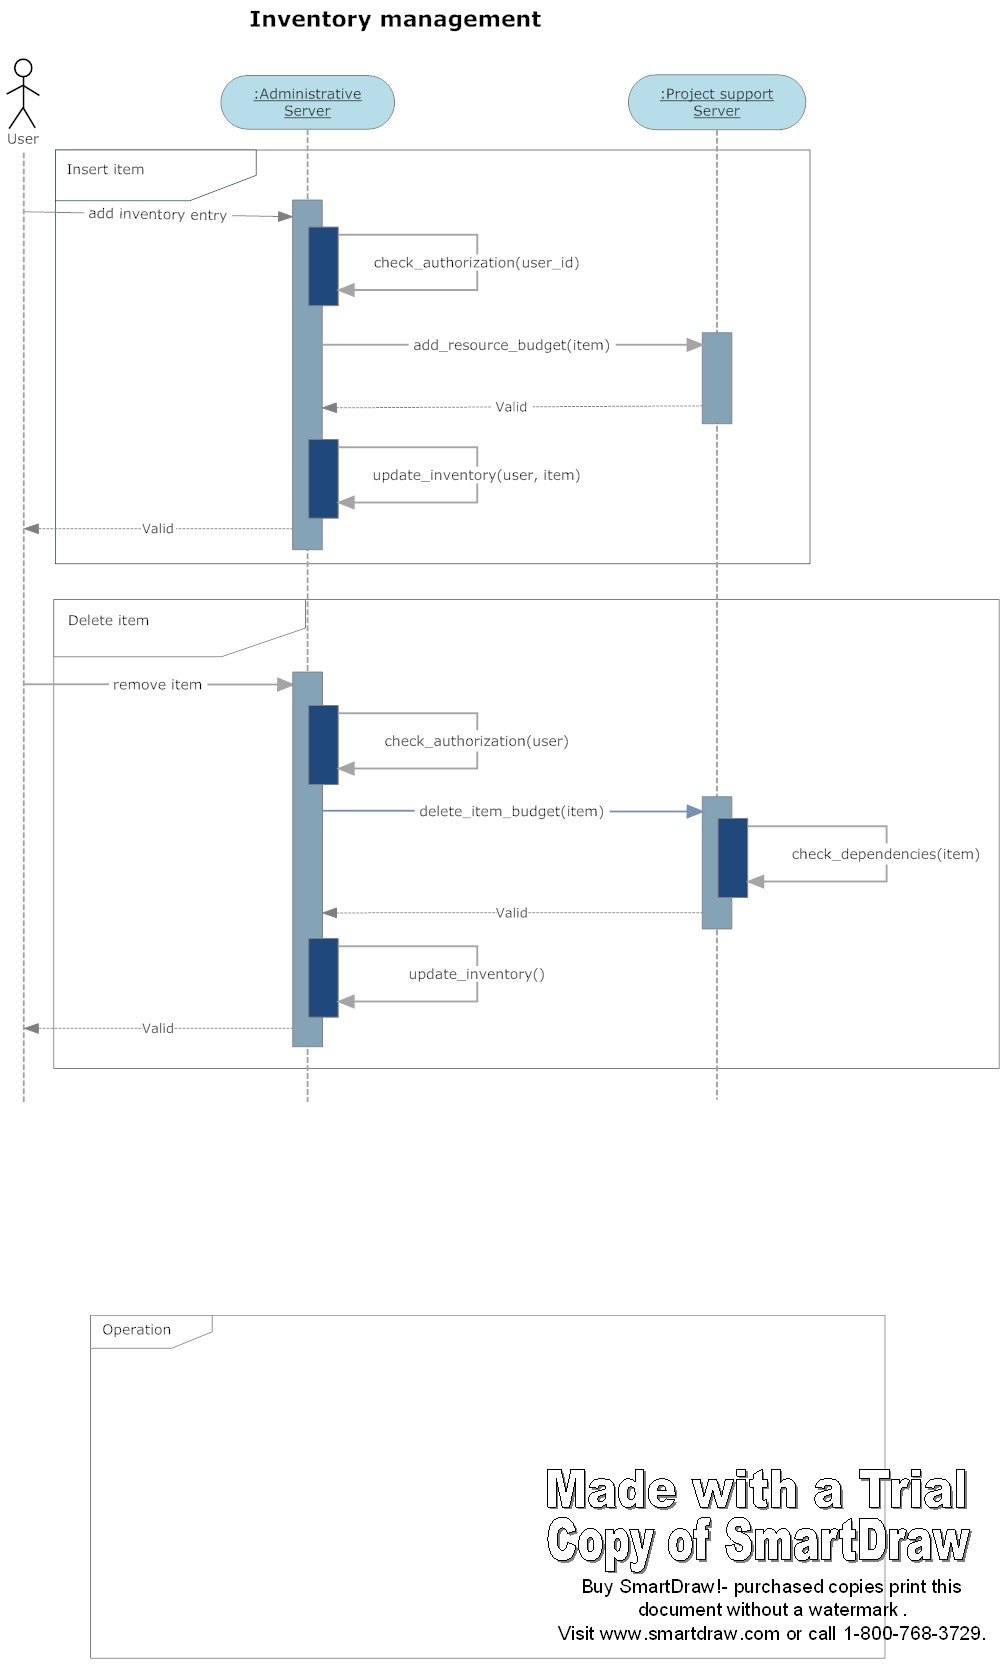
\includegraphics[scale=0.45]{assign3/sdraw/imgs/inventory.jpg}
\caption{Inventory management sequence diagram.}
\label{3img:[sequence]inventory}
\end{centering}
\end{figure}

\subsection{Editing documentation}
\begin{figure}
\begin{centering}
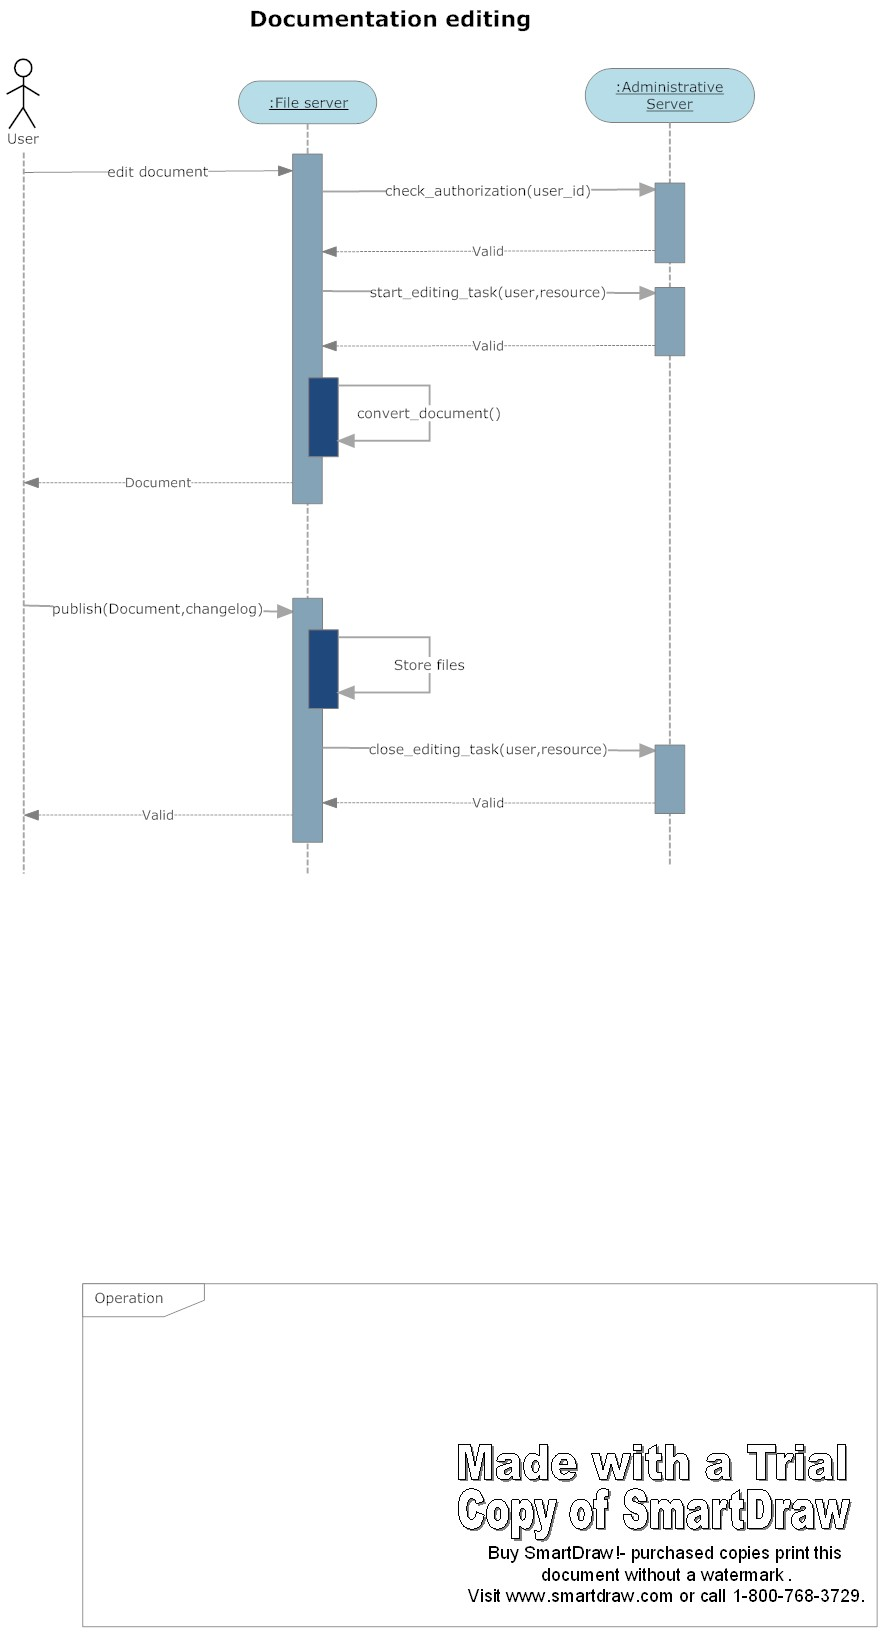
\includegraphics[scale=0.45]{assign3/sdraw/imgs/editing.jpg}
\caption{Editing documentation sequence diagram.}
\label{3img:[sequence]editing}
\end{centering}
\end{figure}</span></div><div class="line" id="LC102"><span class="k">\input</span><span class="nb">{</span>assign2/sections/research<span class="nb">}</span></div><div class="line" id="LC103"><span class="k">\input</span><span class="nb">{</span>assign2/sections/courses<span class="nb">}</span></div><div class="line" id="LC104">&nbsp;</div></pre></div>
            
          </td>
        </tr>
      </table>
    
  </div>


      </div>
    </div>
    
  


  </div>

      
      
      <div class="push"></div>
    </div>
    
    <div id="footer">
      <div class="site">
        <div class="info">
          <div class="links">
            <a href="http://github.com/blog/148-github-shirts-now-available">Shirts</a> |
            <a href="http://github.com/blog">Blog</a> |
            <a href="http://support.github.com/">Support</a> |
            <a href="http://github.com/training">Training</a> |
            <a href="http://github.com/contact">Contact</a> |
            <a href="http://groups.google.com/group/github/">Google Group</a> |
            <a href="http://develop.github.com">API</a> |
            <a href="http://twitter.com/github">Status</a>
          </div>
          <div class="company">
            <span id="_rrt" title="0.36011s from xc88-s00009">GitHub</span>
            is <a href="http://logicalawesome.com/">Logical Awesome</a> &copy;2009 | <a href="/site/terms">Terms of Service</a> | <a href="/site/privacy">Privacy Policy</a>
          </div>
        </div>
        <div class="sponsor">
          <a href="http://engineyard.com"><img src="/images/modules/footer/engine_yard_logo.png" alt="Engine Yard" /></a>
          <div>
            Hosting provided by our<br /> partners at Engine Yard
          </div>
        </div>
      </div>
    </div>
    
    <div id="coming_soon" style="display:none;">
      This feature is coming soon.  Sit tight!
    </div>

    
        <script type="text/javascript">
    var gaJsHost = (("https:" == document.location.protocol) ? "https://ssl." : "http://www.");
    document.write(unescape("%3Cscript src='" + gaJsHost + "google-analytics.com/ga.js' type='text/javascript'%3E%3C/script%3E"));
    </script>
    <script type="text/javascript">
    var pageTracker = _gat._getTracker("UA-3769691-2");
    pageTracker._initData();
    pageTracker._trackPageview();
    </script>

    
  </body>
</html>

